\chapter{機能}\label{cha:Function}
本章では、本研究で試作するモータ特性表自動生成ツールの機能について説明する。

Modelica言語で作成したモータのモデルを、OpenModelicaでシミュレーションした際にcsvファイルが出力される。
今回試作するモータ特性表自動生成ツールは、OpenModelicaが出力したcsvファイルを入力として読み込み、
モータ特性表を出力として生成する。
% \section{ツールの機能}\label{kinou}
% \subsection{モータ特性表生成}\label{sub:kenkyu_mokuteki}
% \vspace{-3zh}
\section{モータ特性表生成}\label{kenkyu_mokuteki}
% 今回試作したモータ特性表自動生成ツールは、次の9個の要素を持つ特性表と4つのグラフを生成する。
今回試作したモータ特性表自動生成ツールは、\ref{mortoku}節で挙げた9個の要素を持つ特性表と、4つの特性グラフを作成し、それらを1つのPDFファイルにまとめ、モータ特性表として出力する。
% \vspace{-3zh}
\section{ツールの実行}\label{zikkou}
% 今回試作したツールの実行方法は、ツールのファイルが存在するディレクトリで、コマンド「python characteristic.py 第1引数 第2引数 第3引数」を実行することである。\\
今回試作したツールを実行するためのコマンドを以下に示す。
% \begin{figure}[t]
% 	\lstinputlisting[]{Image/comand.txt}
% 	\caption{実行コマンド}
% 	\label{lis:zikkoucomand}
% \end{figure}
\begin{figure*}[t]
	\lstinputlisting[label={code:zikkou}, caption={実行コマンド}]{Image/comand.txt}
\end{figure*}
なお、このコマンドは、ツールの実行ファイルが存在するディレクトリで実行する必要がある。

第1引数には、入力とするcsvファイルのパスを含めたファイル名を指定する。

第2引数には、第1引数で指定したcsvファイルの中の、モータ特性表を自動生成したいモータのモデルに含まれる、慣性部品のオブジェクト名を指定する。

第3引数には、第1引数で指定したcsvファイルの中の、モータ特性表を自動生成したいモータのモデルに含まれる、電源部品のオブジェクト名を指定する。

第2引数と、第3引数に慣性部品と電源部品のオブジェクト名を指定する理由については、\ref{syutoku_data}章で述べる。

% 図\ref{fig:tantai_model}のモデルをシミュレーションした時に、OpenModelicaから出力されるcsvファイルの一部を、図\ref{fig:simyu_csv}に示す。\\
図\ref{fig:simyu_csv}のファイル名が、「DCmotor\_res.csv」であり、慣性部品のオブジェクト名が、「inertia1」であり、
電源部品のオブジェクト名が、「signalVoltage1」だった場合の実行コマンドを、図\ref{fig:zikkou}に示す。

モータ特性表が自動生成できた場合は、図\ref{fig:zikkou}に示すように、画面上に「characteristicTable.pdf created」と青色で表示する。

今回試作したツールでは、毎回モータ特性表を「characteristicTable.pdf」で保存するため、同じファイル名がある場合、上書き保存となる。

自動生成できなかった場合については、\ref{error}節で述べる。\\

図\ref{fig:zikkou}のコマンドでツールを実行し、自動生成したモータ特性表を、図\ref{fig:tokuseihyou}に示す。
\begin{figure}[t]
	\centering
	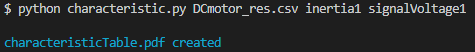
\includegraphics[width=12cm,height=1.5cm]{./Image/succes_comand.png}
	\caption{実行コマンド例}
	\label{fig:zikkou}
\end{figure}
% \clearpage
% \fboxsep=0pt
%  \fbox{
% 	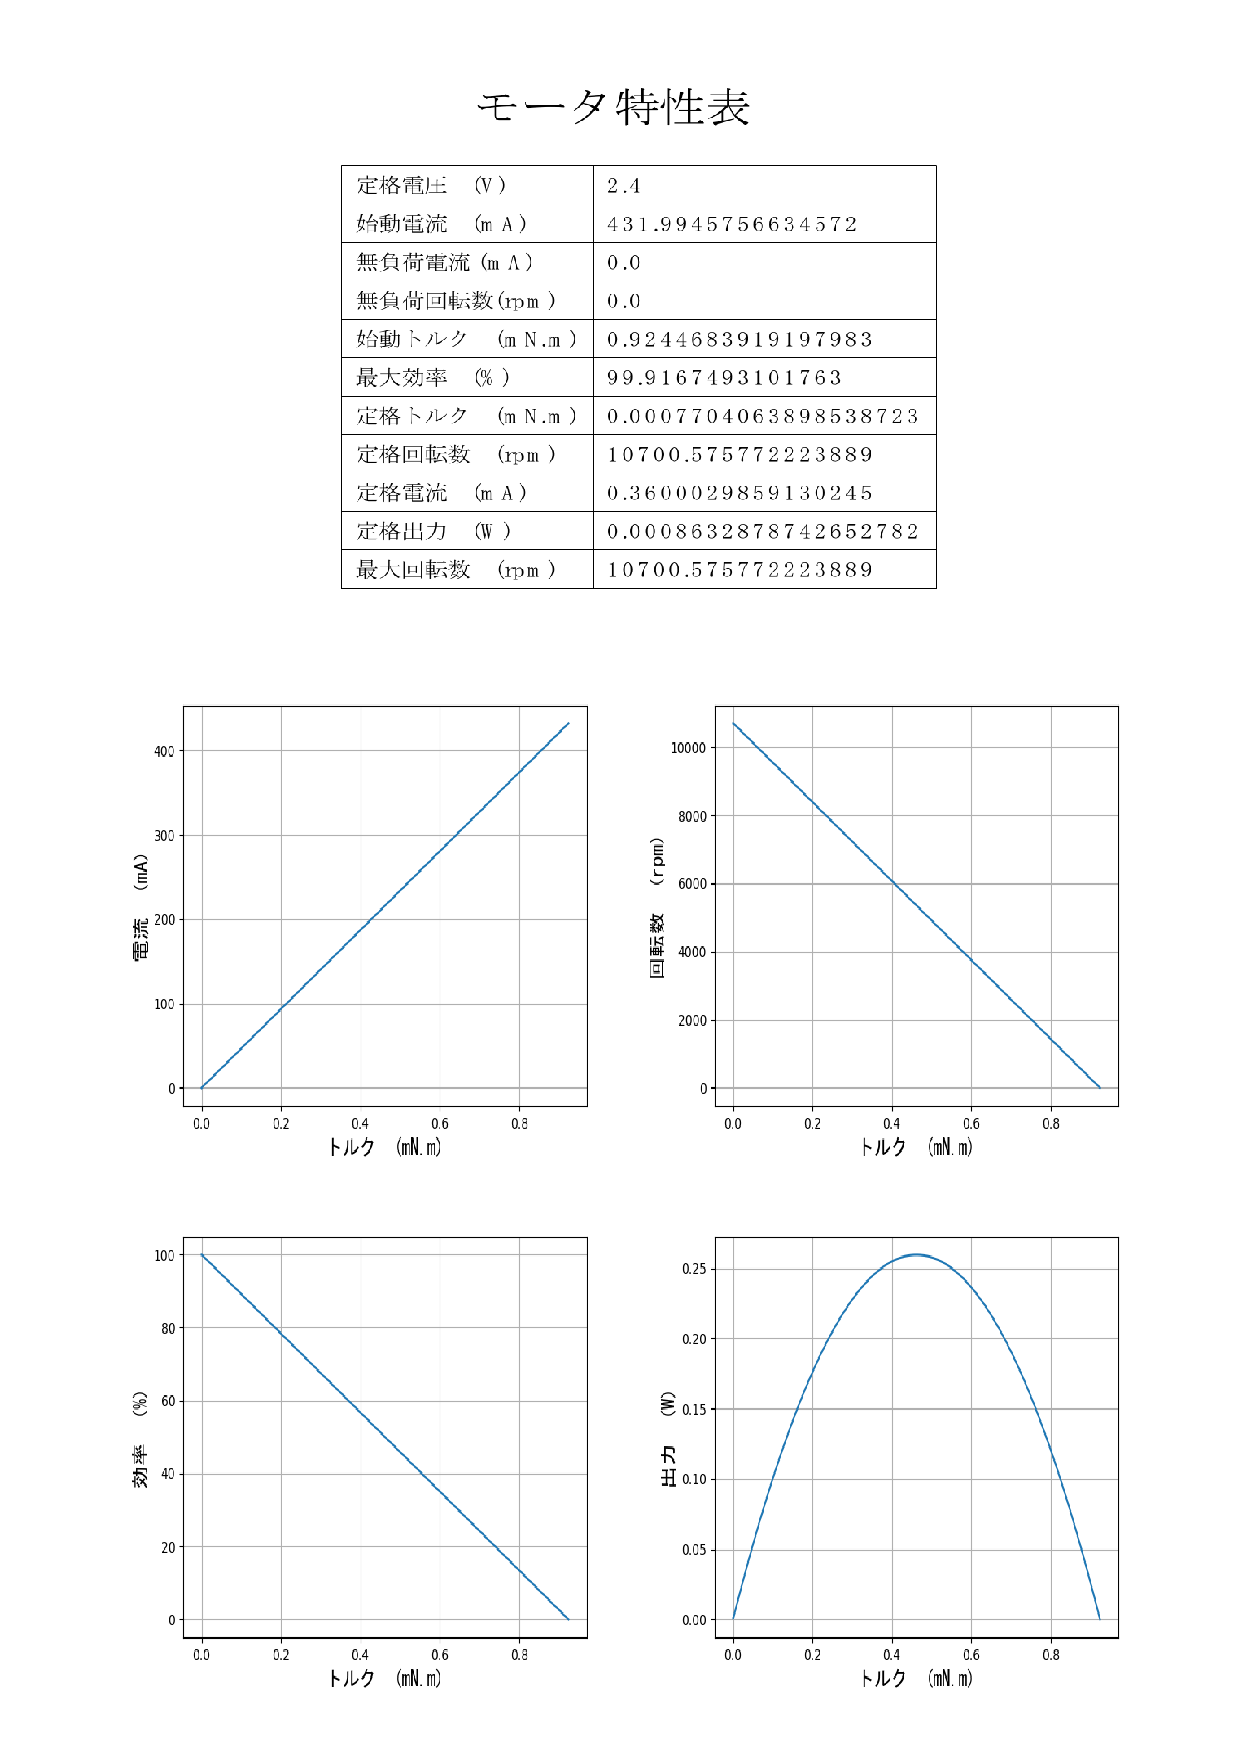
\includegraphics[width=16cm,pagebox=cropbox]{Image/characteristicTable.pdf} 
% 	% \label{fig:tokuseihyou}
%  }
\begin{figure}[t]
	\centering
	\fbox{
	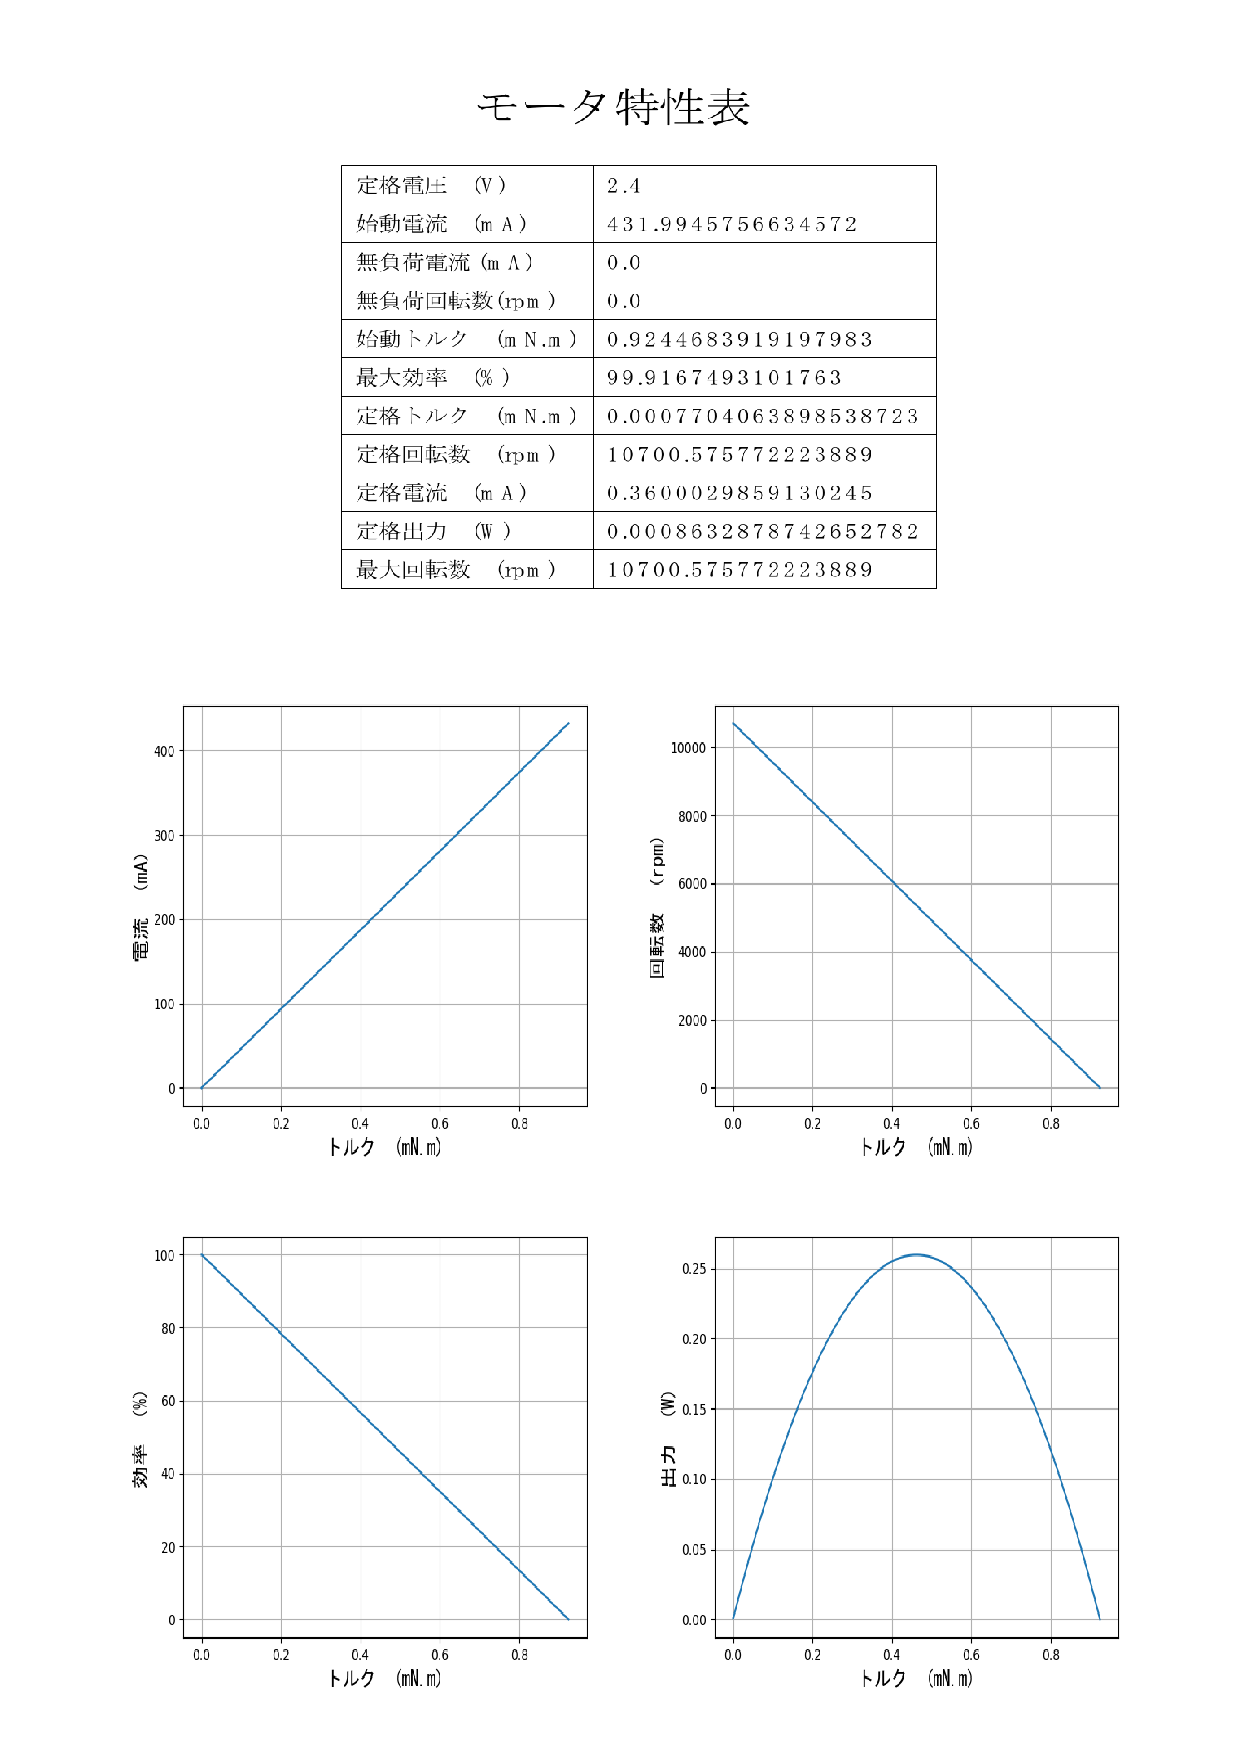
\includegraphics[width=16cm,pagebox=cropbox]{Image/characteristicTable.pdf} 
	}
	\caption{モータ特性表}
	\label{fig:tokuseihyou}
\end{figure}
% \clearpage
% \subsection{実行コマンド}\label{sub:comand}
% \vspace{-5zh}
% \subsection{エラー表示}\label{sub:error}
\section{エラー表示}\label{error}
\ref{zikkou}節で、試作したツールを実行するためのコマンドは、「python characteristic.py 第1引数 第2引数 第3引数」であると述べた。
このコマンドを実行した際に、モータ特性表が自動生成できなかった場合は、原因が3つ考えられる。

1つ目の原因は、引数の数が足りていない、もしくは多い場合である。\\
この場合は、エラー文として「ERROR : 引数の数が間違っています」を、赤色で画面上に表示する。
この例を、図\ref{fig:error_hikisuu}に示す。

2つ目の原因は、第1引数で指定したcsvファイルのファイル名が間違っている場合である。

この場合は、エラー文として「ERROR : 指定したファイル名が間違っています」を、赤色で画面上に表示する。
この例を、図\ref{fig:error_file}に示す。

3つ目の原因は、第2引数と第3引数のどちらか一方、もしくはその両方に間違いがあった場合である。

この場合は、エラー文として「ERROR : 指定したオブジェクト名が違います」を、赤色で画面上に表示する。
この例を、図\ref{fig:error_comand}に示す。

上記3つの原因にすべて該当するコマンドの場合は、第1引数から順に処理を行い、エラーがあればそこで処理を止めるため、図\ref{fig:error_hikisuu}のエラー文のみ表示する。

\begin{figure}[t]
	\centering
	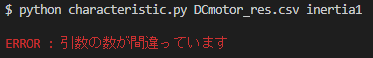
\includegraphics[width=10cm,height=1.5cm]{./Image/error_tarinai.png}
	\caption{引数の数に誤りがあった場合のエラー分の例}
	\label{fig:error_hikisuu}
\end{figure}

\begin{figure}[t]
	\centering
	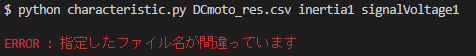
\includegraphics[width=12cm,height=1.5cm]{./Image/error_file.png}
	\caption{第1引数に誤りがあった場合のエラー文の例}
	\label{fig:error_file}
\end{figure}

\begin{figure}[t]
	\centering
	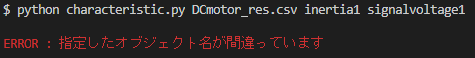
\includegraphics[width=12cm,height=1.5cm]{./Image/error_comand.png}
	\caption{第2引数、第3引数に誤りがあった場合のエラー文の例}
	\label{fig:error_comand}
\end{figure}